\documentclass[a4paper,12pt,oneside]{scrartcl}

% Setup page
\usepackage[top=2.0cm, bottom=2.0cm, left=3cm, right=1.5cm, footskip=0.5cm]{geometry}
\usepackage{epsfig}
\usepackage{xcolor}

% Base packages
\usepackage{fontspec}
\usepackage{booktabs}
\usepackage{xunicode}
\usepackage{xltxtra}
\usepackage{comment}
\usepackage{amsfonts}
\usepackage{amsmath}
\usepackage{longtable}
\usepackage{csquotes}
\usepackage{setspace}
\usepackage{placeins}
\usepackage{float}
\setcounter{tocdepth}{4}
\setcounter{secnumdepth}{4}
% Setup Russian hyphenation
\usepackage{polyglossia}
\setdefaultlanguage[spelling=modern]{russian} % for polyglossia
\setotherlanguage{english} % for polyglossia
\defaultfontfeatures{Scale=MatchLowercase, Mapping=tex-text}

% Setup fonts
\newfontfamily\russianfont{CMU Serif}
\newfontfamily\cyrillicfont{CMU Serif}
\setromanfont{CMU Serif}
\setsansfont{CMU Sans Serif}
\setmonofont{CMU Typewriter Text}


% Be able to include PNG and PDF as images
\usepackage{graphicx}
\usepackage{subcaption}

% Be able to insert hyperlinks
\usepackage{hyperref}
\hypersetup{colorlinks=true, linkcolor=black, filecolor=black, citecolor=black, urlcolor=black , pdfauthor=Zakharov Pavel <paltoszaharov@phystech.edu>, pdftitle=Диплом_бакалавриат}
\usepackage{url}

% Misc optional packages
\usepackage{footnpag}
\usepackage{indentfirst}
\usepackage{underscore}
\usepackage{amsthm}
\usepackage{enumitem} % continue enumeration 
\usepackage{mdwlist} % compact itemize lists environment
\usepackage{mdwlist} % compact itemize lists environment
%\renewcommand{\labelitemi}{--}  % Use endash for itemized lists
\usepackage[hang,flushmargin]{footmisc} % correct indent for footnotes


% Attach TikZ/PGF system to be able to draw vector plots.
% \usepackage{tikz}
% \usetikzlibrary{shapes, calc, arrows, fit, positioning, decorations, patterns, decorations.pathreplacing,chains, snakes}

% A new command to mark not done places
\newcommand{\todo}[1]{{\color{red}TODO\ #1}}
\onehalfspacing
\begin{document}

\begin{titlepage}
\thispagestyle{empty}

{\centering
Федеральное государственное автономное образовательное учреждение высшего образования 
<<Московский физико{}-технический институт (государственный университет)>>\par}

\bigskip
{\centering
Физтех-школа радиотехники и компьютерных технологий \par}

\bigskip
{\centering 
Кафедра микропроцессорных технологий в интеллектуальных системах управления
\par}

%\endhead

\bigskip

\bigskip


\vfill

{\centering\Large\bfseries
\textbf{Исследование мультиантенных систем в применении к беспроводным сенсорным сетям}
\par}

\bigskip

{\centering\bfseries
Выпускная квалификационная работа

(бакалаврская работа)

\bigskip
Направление подготовки: 03.03.01 Прикладные математика и физика
\par}

\vfill

\begin{tabular}{lll}\\
\specialcell{Выполнил:\\студент 516 группы}  & ______________ & Захаров Павел Сергеевич \\
                     &                &                  \\
Научный руководитель: & ______________ & Владимиров Леонид Леонидович \\
\end{tabular}

\vfill

{\centering
Москва 
2019
\par}

\end{titlepage}

\cleardoublepage


\tableofcontents
\listoffigures
\listoftables

\cleardoublepage

\section{Введение}
Развитие микроэлектроники позволило наладить производство дешевых и экономичных устройств передачи данных, сенсоров и микроконтроллеров. Их появление привело к развитию беспроводных сенсорных сетей (Wireless Sensor Networks, или WSN), которые позволяют организовать автоматизированный сбор данных с больших территорий без необходимости разворачивать громоздкую инфраструктуру в виде кабелей передачи данных, проводов питания и т.д. Они применяются в промышленности, жилищно-коммунальном хозяйстве, городской инфраструктуре, экологических и метеорологических исследованиях, системах охраны и многих других отраслях.

\begin{figure}[!htb]
    \centering
    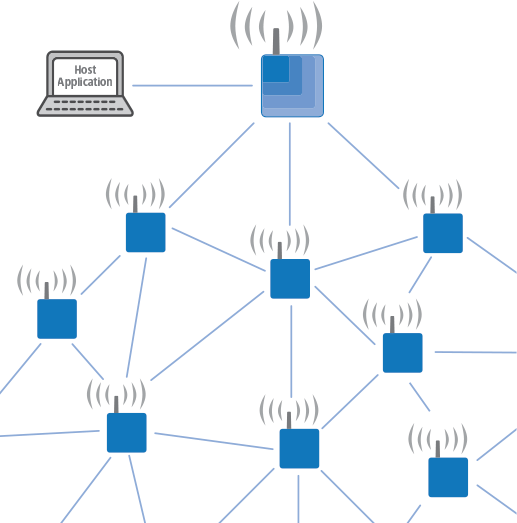
\includegraphics[width=0.6\textwidth]{pics/1.png}
    \caption{Общая схема беспроводной сенсорной сети}
    \label{fig:WSN}
\end{figure}

Такие сети, как правило, состоят из базовых станций, осуществляющих сбор данных с подчиненных им датчиков (узлов). Сенсоры, однако, не могут использовать высокие мощности передатчика ввиду регуляторных ограничений и необходимости обеспечить как можно больший срок работы от батареи. Из-за этого установление радиоканала между датчиком и базовой станцией может быть затруднено. Для решения возникшей проблемы используются технологии ретрансляции, которые позволяют устройствам в сети кооперироваться при передаче данных \cite{B1}.

Обычно в подобных сетях одна базовая станция; соответственно, кооперируются обычно узлы сети. Однако в многоквартирных домах нередко создается отдельная сеть для каждой квартиры со своей базовой станцией. Нередко эта базовая станция сама является сенсором. При этом базовые станции могут быть связаны альтернативным каналом связи (PLC или традиционные кабели). Это позволяет использовать антенны базовых станций для связи с конкретным узлом, фактически выстраивая виртуальную мультиантенную систему. В таком случае используются соответствующие методы обработки сигналов. Тем не менее, в сенсорных сетях антенны все-таки принадлежат различным устройствам, что ставит перед разработчиками дополнительные задачи по синхронизации и обмену информацией. Данная работа посвящена анализу применимости подобных методов комбинирования сигналов от разных устройств применительно к беспроводным сенсорным сетям.

\clearpage

\section{Обзор литературы}
\subsection{Общая схема}
Что-нибудь

Кооперация между базовыми станциями занимает промежуточное положение между обычными мультиантенными системами и WSN с кооперативной передачей данных от узлов: с одной стороны, базовые станции все еще являются отдельными устройствами, и поэтому имеют разные осцилляторы, тактовые сигналы и т.п. Это порождает проблемы, характерные для WSN, однако взаимодействие и синхронизация между базовыми станциями могут быть упрощено ввиду наличия альтернативных каналов связи и большей вычислительной мощности базовых станций. При этом восходящее (к базовым станциям) и нисходящее (к узлам) направления связи отличаются по требовательности к синхронизации и рассматриваются отдельно.

\subsection{Восходящая линия связи}

При передаче данных на базовые станции они независимо друг от друга принимают и оцифровывают сигнал. Далее происходит обработка \Large baseband \normalsize сигналов, их комбинирование. Происходящее принципиально не отличается от стандартных методов обработки пространственно разнесенных сигналов...

\subsection{Нисходящая линия связи}

В случае нисходящей линии связи базовые станции отправляют данные так, чтобы сигналы пришли на антенну узла в фазе и таким образом усилились. Решить эту задачу позволяют наработки по кооперативной передаче данных..


Andreas F. Molisch в \cite{B1} приводит следующую классификацию методов ретрансляции:
\begin{enumerate}
\item \textit{Multi-hop} - последовательная пересылка данных от узла к узлу, пока информация не дойдет до базовой станции;
\item \textit{Split-Combine} - рассылка данных доступным узлам, а затем коллективная одновременная передача на базовую станцию;
\item \textit{Diversity} - сначала источник рассылает данные узлам и базовой станции, затем узлы еще раз передают ту же информацию на базовую станцию;
\item \textit{Nonorthogonal Diversity} -  
\end{enumerate}
\clearpage


%\section{Разрабатываемый ПНЧ}
%
%С целью создания систем прецизионного непрерывного мониторинга аналоговых сигналов поставлена задача разработки многоканального ПНЧ, удовлетворяющего повышенным требованиям по точностным и скоростным параметрам. Ниже приведены требования к интегратору разрабатываемого ПНЧ. Поскольку точностные параметры ПНЧ определяются параметрами усилителя интегратора, для оценки соответствия параметров разрабатываемого усилителя требованиям ПНЧ рассмотрим подробно параметры ПНЧ и интегратора.
%
%
%
%
%
%\subsection{Параметры ПНЧ}\label{sec:parameters}
%
%Целевые требования к параметрам интегратора, определяемые требованиями ТЗ на микросхему ПНЧ представлены в таблице Таблица~\ref{fig:Table2}. Целевые требования к параметрам интегратора определены с учетом технологического запаса 100\%.
%
%
%В таблице~\ref{fig:Table3} приведены предельный и предельно-допустимый режимы эксплуатации ПНЧ.
%
%
%Требуемую совокупность параметров можно обеспечить   только в синхронном балансирующем ПНЧ, позволяющем достичь максимальной точности и стабильности преобразования. 
%
%%\begin{figure}[!htb]
%%    \centering
%%    \includegraphics[width=0.6\textwidth]{pics/pic1.png}
%%    \caption{Узел БСС с использованием: a) АЦП (ADC) б) ПНЧ (VFC)}
%%    \label{fig:WSN}
%%\end{figure}
%
%
%
%
%
%\subsection{Структурная схема канала разрабатываемого ПНЧ}
%
%Рассмотрим структурную схему канала ПНЧ - Рисунок~\ref{fig:VFC}. 
%
%Основой канала интегрирующего преобразователя напряжения в частоту (ПНЧ) является интегратор, включающий усилитель ОУ с конденсатором обратной связи $C_{int}$ и резистивно-ключевая схема коммутации входа интегратора int\_sw. 
%
%Положительное опорное напряжение $V_{ref}$ можно использовать как внешнее, так и внутреннее. Номинальная величина опорного напряжения $V_{ref}$ = 1.25 В.  Инвертирующий операционный усилитель формирует общее для всех каналов отрицательное опорное напряжение  $V_{refb}$ = -1.25В. Буферные усилители с подстройкой смещения нуля в каждом канале формируют индивидуально калибруемые отрицательные опорные напряжения $V_{refb_{i}}$. 
%
%В нормальном режиме напряжение на входе In преобразуется в ток и попадает на вход интегратораи увеличивая или уменьшая выходное напряжение интегратора, в зависимости от полярности входного напряжения Если напряжение выхода интегратора превысит $V_{ref}$ то сработает компаратор CpT и откроет ключ SwT. Аналогично, если напряжение выхода интегратора будет меньше $V_{refb}$ сработает компаратор CpB и откроет ключ SwB. Сигналы ft, fb управления ключами синхронизуются передним фронтом тактового сигнала $F_{clk}$. 
%
%
%
%\section{Заключение}
%
%Целью данной работы была разработка прецезионного операционного усилителя для интегратора ПНЧ. В разработке использовалось известное техническое решение, минимизирующие смещение нуля - чопперная-стабилизация. Дополнительно предложено введение динамической калибровки для повышения точности ПНЧ. Чопперная-стабилизация уменьшает смещение создаваемое 1 каскадом. Динамическая калибровка уменьшает нелинейность вносимую ключами чоппера, а также выходного каскада. В результате моделирования ОУ были получены его основные характеристики, которые представлены в таблице~\ref{comp}.
%
%
%Данные таблицы показывают, что полученные характеристики ОУ интегратора обеспечивают требуемые точностные праметры ПНЧ.





%==========================================================

\cleardoublepage
\begin{thebibliography}{99}
\bibitem{B1} Andreas F. Molisch, “Wireless Communications” 2nd edition, John Wiley \& Sons, 2011.
\bibitem{B2} Paul Klonowski, "Analog-to-Digital Conversion Using Voltage-to-Frequency Converters," Application Note AN-276, Analog Devices, Inc. (a good application note on VFCs).
\bibitem{B3} Cristina Azcona Murillo, Belén Calvo Lopez, and Santiago Celma. Pueyo. 2013. Voltage-to-Frequency Converters CMOS Design and Implementation, New York, NY: Springer New York.
\bibitem{B7}Аналоговая электроника: [учеб. пособие], Автор:	Анатолий Леонидович Ларин
Издатель: МФТИ, 2007; ISBN:	5741701833, 9785741701836
\end{thebibliography}

\addcontentsline{toc}{section}{Список литературы}
%=====================================================
\cleardoublepage

\end{document}

